\chapter{Leçon 23: D'Sprangprozessioun}

\noindent\textit{Ce texte est une adaptation par Odile d'une légende luxembourgeoise traditionnelle. / This text is an adaptation by Odile of a traditional Luxembourgish legend.}\\
\noindent\textbf{Source / Sources:} Gredt, Nikolaus: Sagenschatz des Luxemburger Landes 1. Neudruck Esch-Alzette: Kremer-Muller \& Cie, 1963, S. 371-372. \\
\noindent\textbf{Permalink:} \texttt{http://www.zeno.org/nid/20007870051}

\vspace{1em}

\section[De Laange Veit a säi Pilgerwee]{De Laange Veit a säi Pilgerwee \\/ Le Grand Veit et son pèlerinage \\/ The Tall Veit and his pilgrimage}

\noindent\textbf{Zu der Zäit vum hellege Willibrord huet e jonke Mann zu Iechternach gewunnt. Säin Numm war Veit, a well hien sou grouss war, gouf hien och "de Laange Veit" genannt. Hie war, zesummen mat senger Fra, viru kuerzem, zum Chrëschtentum iwwergetrueden an si waren an d'Hellegt Land gepilgert. Et waren elo schonns 10 Joer vergaangen, dass si fort waren, a well an Iechternach kee méi eppes vun hinnen héieren hat, hunn d'Leit geduecht, si wieren gestuerwen. Doropshin huet hir Famill all hir Saachen ënnert sech opgedeelt. Et war eng grouss Iwwerraschung, wéi, am Joer 729 op Ouschteren, de Laange Veit onverhofft rëm zu Iechternach opgetaucht ass. Awer, a sengem Gesiicht, wat soss ëmmer sou gestraalt huet, stoung Trauer: Seng gutt Fra war op der laanger Rees gestuerwen. Si war souguer ëmbruecht ginn. An hie selwer hat guer näischt méi, ausser engem komeschen, onbekannten Instrument: enger Gei.}\\[1.5em]

\begin{center}
    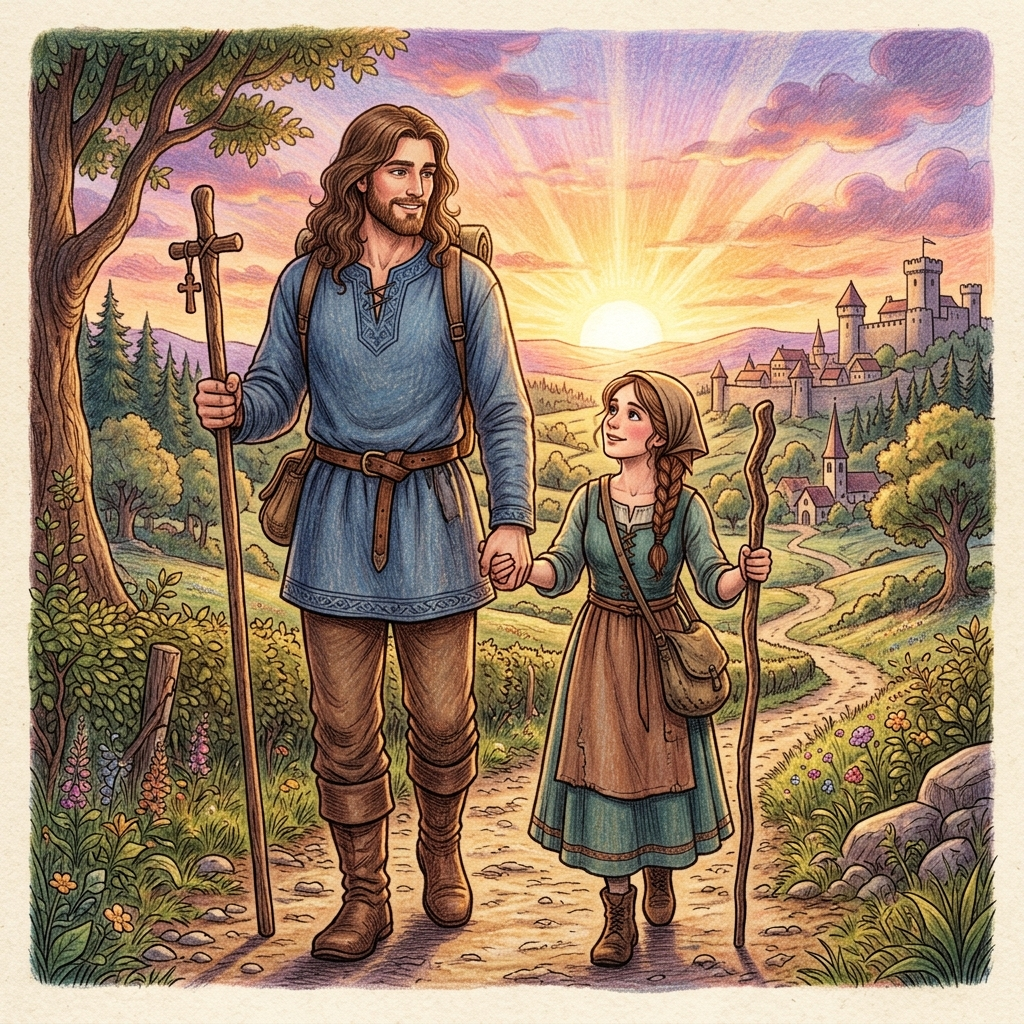
\includegraphics[width=0.6\linewidth]{vokab_300dpi/pilger_wee.png} \\
    \small\textit{De Veit a seng Fra um Pilgerwee / Veit et son épouse en pèlerinage / Veit and his wife on pilgrimage}
\end{center}


\textbf{1. Zu der Zäit vum hellege Willibrord huet e jonke Mann zu Iechternach gewunnt.}\\
\textit{Zu der Zäit} (À l'époque / At the time) \textit{vum} (du / of the) \textit{hellege Willibrord} (saint Willibrord) \textit{huet... gewunnt} (vivait / lived - past of \textit{wunnen}) \textit{e jonke Mann} (un jeune homme / a young man) \textit{zu Iechternach} (à Echternach / in Echternach).\\
$\rightarrow$ Français : À l'époque de saint Willibrord, un jeune homme vivait à Echternach.\\
$\rightarrow$ English : At the time of Saint Willibrord, a young man lived in Echternach.\\[0.5em]

\textbf{2. Säin Numm war Veit, a well hien sou grouss war, gouf hien och "de Laange Veit" genannt.}\\
\textit{Säin Numm} (Son nom / His name) \textit{war Veit} (était Veit / was Veit), \textit{a well} (et parce que / and because) \textit{hien} (il / he) \textit{sou} (si / so) \textit{grouss} (grand / tall) \textit{war} (était / was), \textit{gouf hien och... genannt} (fut-il aussi appelé / was he also called).\\
$\rightarrow$ Français : Son nom était Veit, et comme il était si grand, on l'appelait aussi « le Grand Veit » (le Long Veit).\\
$\rightarrow$ English : His name was Veit, and because he was so tall, he was also called "the Tall Veit" (the Long Veit).\\[0.5em]

\textbf{3. Hie war, zesummen mat senger Fra, viru kuerzem, zum Chrëschtentum iwwergetrueden an si waren an d'Hellegt Land gepilgert.}\\
\textit{Hie war} (Il était / He was), \textit{zesummen} (ensemble / together) \textit{mat senger Fra} (avec sa femme / with his wife), \textit{viru kuerzem} (récemment / recently) \textit{zum Chrëschtentum} (au christianisme / to Christianity) \textit{iwwergetrueden} (converti / converted - past participle of \textit{iwwertrieden}), \textit{an} (et / and), \textit{si waren gepilgert} (ils étaient partis en pèlerinage / they had gone on a pilgrimage), \textit{an d'Hellegt Land} (en Terre sainte / to the Holy Land).\\
$\rightarrow$ Français : Il s'était récemment converti au christianisme avec sa femme, et ils étaient partis en pèlerinage en Terre sainte.\\
$\rightarrow$ English : He had recently converted to Christianity together with his wife, and they had gone on a pilgrimage to the Holy Land.\\[0.5em]

\textbf{4. Et waren elo schonns 10 Joer vergaangen, dass si fort waren, a well an Iechternach kee méi eppes vun hinnen héieren hat, hunn d'Leit geduecht, si wieren gestuerwen.}\\
\textit{Et waren elo schonns} (Il y avait maintenant déjà / There were now already) \textit{10 Joer vergaangen} (10 ans passés / 10 years passed), \textit{dass} (que / that) \textit{si fort waren} (ils étaient partis / they were gone), \textit{a well} (et comme / and because) \textit{an Iechternach} (à Echternach / in Echternach) \textit{kee méi eppes} (plus personne / no one anymore anything) \textit{vun hinnen} (d'eux / of them) \textit{héieren hat} (avait entendu / had heard), \textit{hunn d'Leit geduecht} (les gens ont pensé / people thought), \textit{si wieren gestuerwen} (qu'ils étaient morts / they had died).\\
$\rightarrow$ Français : Dix ans s'étaient déjà écoulés depuis leur départ, et comme personne à Echternach n'avait plus eu de leurs nouvelles, les gens pensaient qu'ils étaient morts.\\
$\rightarrow$ English : Ten years had already passed since they had left, and because no one in Echternach had heard anything of them anymore, people thought they had died.\\[0.5em]

\textbf{5. Doropshin huet hir Famill all hir Saachen ënnert sech opgedeelt.}\\
\textit{Doropshin} (Là-dessus / Thereupon), \textit{huet hir Famill} (leur famille a / their family did - referring to the family of him and his wife), \textit{all hir Saachen} (toutes leurs affaires / all their things) \textit{ënnert sech} (entre eux / among themselves) \textit{opgedeelt} (partagé / divided).\\
$\rightarrow$ Français : Là-dessus, leur famille a partagé toutes leurs affaires entre eux.\\
$\rightarrow$ English : Thereupon, their family divided all their things among themselves.\\[0.5em]

\textbf{6. Et war eng grouss Iwwerraschung, wéi, am Joer 729 op Ouschteren, de Laange Veit onverhofft rëm zu Iechternach opgetaucht ass.}\\
\textit{Et war} (C'était / It was) \textit{eng grouss Iwwerraschung} (une grande surprise / a great surprise), \textit{wéi} (quand / when), \textit{op Ouschteren} (à Pâques / at Easter), \textit{de Laange Veit} (le Grand Veit / the Tall Veit) \textit{onverhofft} (de manière inattendue / unexpectedly) \textit{rëm} (de retour / back again) \textit{zu Iechternach} (à Echternach / in Echternach) \textit{opgetaucht ass} (est apparu / appeared).\\
$\rightarrow$ Français : Ce fut une grande surprise lorsque, le jour de Pâques de l'an 729, le Grand Veit est réapparu de manière inattendue à Echternach.\\
$\rightarrow$ English : It was a great surprise when, on Easter Day in the year 729, the Tall Veit unexpectedly reappeared in Echternach.\\[0.5em]

\textbf{7. Awer, a sengem Gesiicht, wat soss ëmmer sou gestraalt huet, stoung Trauer: Seng gutt Fra war op der laanger Rees gestuerwen.}\\
\textit{Awer, a sengem Gesiicht} (Mais sur son visage / But on his face), \textit{wat soss ëmmer} (qui d'habitude toujours / which usually always) \textit{sou} (si / so) \textit{gestraalt huet} (rayonnait / beamed), \textit{stoung Trauer} (se lisait la tristesse / stood sadness): \textit{Seng gutt Fra} (sa bonne épouse / his good wife) \textit{war gestuerwen} (était morte / had died) \textit{op der laanger Rees} (pendant le long voyage / on the long journey).\\
$\rightarrow$ Français : Mais sur son visage, qui d'habitude rayonnait tant, se lisait la tristesse : sa bonne épouse était morte pendant le long voyage.\\
$\rightarrow$ English : But on his face, which usually beamed so much, stood sadness: His good wife had died on the long journey.\\[0.5em]

\textbf{8. Si war souguer ëmbruecht ginn.}\\
\textit{Si war} (Elle était / She was) \textit{souguer} (même / even) \textit{ëmbruecht ginn} (été tuée, assassinée / been killed - passive past).\\
$\rightarrow$ Français : Elle avait même été assassinée.\\
$\rightarrow$ English : She had even been murdered.\\[0.5em]

\textbf{9. An hie selwer hat guer näischt méi, ausser engem komeschen, onbekannten Instrument: enger Gei.}\\
\textit{An hie selwer} (Et lui-même / And he himself) \textit{hat} (avait / had) \textit{guer näischt méi} (plus rien du tout / nothing left at all), \textit{ausser} (sauf, à l'exception de / except for) \textit{engem komeschen, onbekannten Instrument} (un instrument étrange et inconnu / a strange, unknown instrument): \textit{enger Gei} (un violon / a violin - dative form of \textit{eng Gei}).\\
$\rightarrow$ Français : Et lui-même n'avait plus rien du tout, à l'exception d'un instrument étrange et inconnu : un violon.\\
$\rightarrow$ English : And he himself had nothing left at all, except for a strange, unknown instrument: a violin.




\section[D'Uklo an den Duell]{D'Uklo an den Duell \\/ L'Accusation et le Duel \\/ The Accusation and the Duel}

\noindent\textbf{Natierlech wollt de Veit säi Besëtz rëm zréck hunn, an dofir huet seng Famill beschloss hien als Mäerder unzekloen: Hien hätt seng Fra op der Rees ermuert. Zu der Zäit war et de Gebrauch, dass esou eng Uklo duerch en Zweekampf ënnerstëtzt ginn ass. Dësen Duell huet op Péngschtméindeg stattfonnt. Dräi der stäerkste Männer haten sech bereet erkläert fir géint de Veit unzetrieden. Schonns an der 1. Ronn, goung hien zu Buedem. Wéi säi Géigner him dunn och nach de Fouss op d'Guergel gedréckt huet, huet hie missen opginn.}\\[1.5em]

\begin{center}
    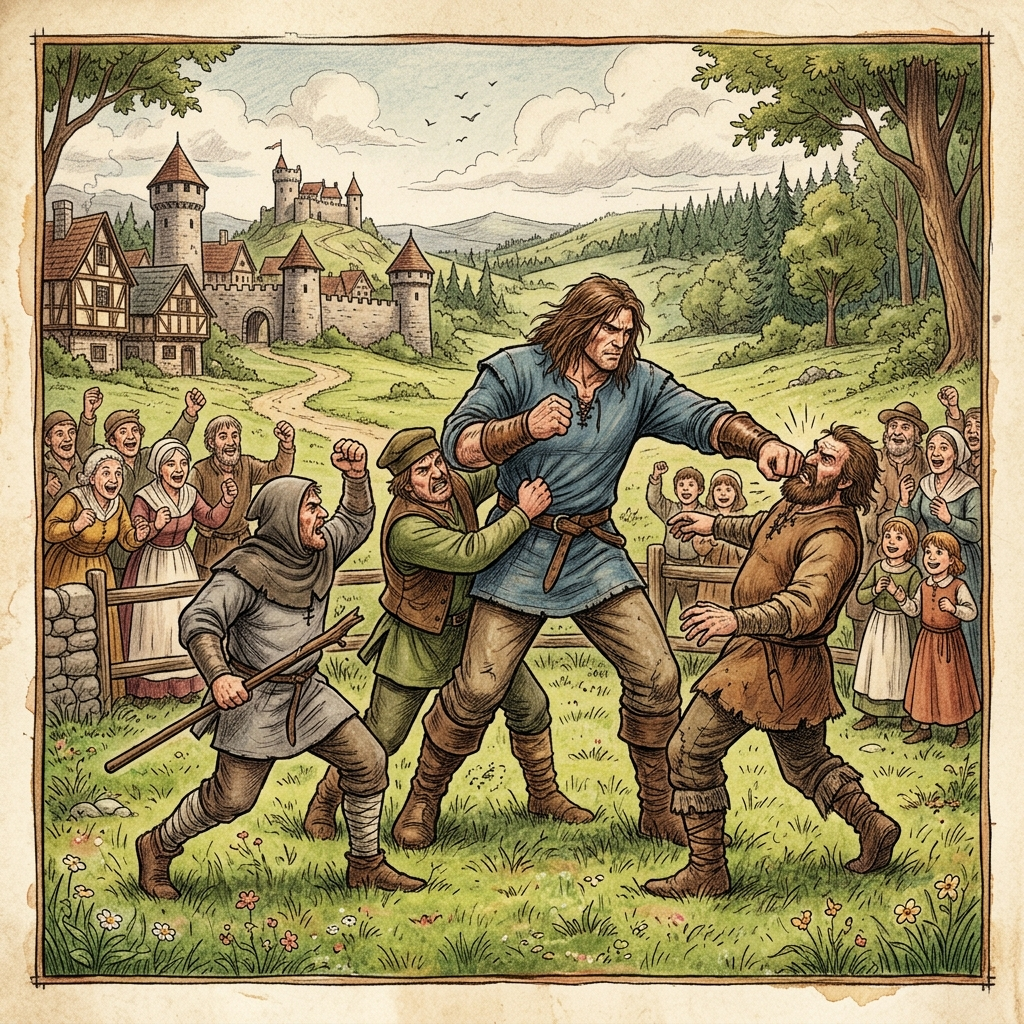
\includegraphics[width=0.6\linewidth]{vokab_300dpi/duell_szene.png} \\
    \small\textit{Den Zweekampf vum Veit géint dräi stäerkste Männer / Le duel de Veit contre trois hommes forts / Veit's duel against three strong men}
\end{center}


\textbf{10. Natierlech wollt de Veit säi Besëtz rëm zréck hunn, an dofir huet seng Famill beschloss hien als Mäerder unzekloen: Hien hätt seng Fra op der Rees ermuert.}\\
\textit{Natierlech wollt de Veit} (Naturellement, Veit voulait / Naturally, Veit wanted), \textit{säi Besëtz} (ses biens / his property) \textit{rëm} (de retour / back) \textit{zréck hunn} (récupérer / to have back), \textit{an dofir} (et c'est pourquoi / and therefore) \textit{huet seng Famill beschloss} (sa famille a décidé / his family decided) \textit{hien... unzekloen} (de l'accuser / to accuse him), \textit{Hien hätt... ermuert} (il aurait assassiné / he had murdered - subjunctive).\\
$\rightarrow$ Français : Naturellement, Veit voulait récupérer ses biens, et c'est pourquoi sa famille a décidé de l'accuser de meurtre : il aurait assassiné sa femme pendant le voyage.\\
$\rightarrow$ English : Naturally, Veit wanted his property back, and therefore his family decided to accuse him of murder: he had allegedly murdered his wife on the journey.\\[0.5em]

\textbf{11. Zu der Zäit war et de Gebrauch, dass esou eng Uklo duerch en Zweekampf ënnerstëtzt ginn ass.}\\
\textit{Zu der Zäit} (À l'époque / At that time) \textit{war et de Gebrauch} (c'était l'usage / it was the custom), \textit{dass} (que / that) \textit{esou eng Uklo} (une telle accusation / such an accusation) \textit{duerch en Zweekampf} (par un duel / by a duel) \textit{ënnerstëtzt ginn ass} (était appuyée / was supported - passive voice).\\
$\rightarrow$ Français : À l'époque, il était d'usage qu'une telle accusation soit appuyée par un duel.\\
$\rightarrow$ English : At that time, it was the custom for such an accusation to be supported by a duel.\\[0.5em]

\textbf{12. Dësen Duell huet op Péngschtméindeg stattfonnt.}\\
\textit{Dësen Duell} (Ce duel / This duel - masculine), \textit{huet... stattfonnt} (a eu lieu / took place), \textit{op Péngschtméindeg} (le lundi de Pentecôte / Whit Monday).\\
$\rightarrow$ Français : Ce duel a eu lieu le lundi de Pentecôte.\\
$\rightarrow$ English : This duel took place on Whit Monday.\\[0.5em]

\textbf{13. Dräi der stäerkste Männer haten sech bereet erkläert fir géint de Veit unzetrieden.}\\
\textit{Dräi der stäerkste Männer} (Trois des hommes les plus forts / Three of the strongest men) \textit{haten sech... erkläert} (s'étaient déclarés / had declared themselves) \textit{bereet} (prêts / ready) \textit{fir... unzetrieden} (à affronter, à combattre / to stand up, compete) \textit{géint de Veit} (contre Veit / against Veit).\\
$\rightarrow$ Français : Trois des hommes les plus forts s'étaient déclarés prêts à affronter Veit.\\
$\rightarrow$ English : Three of the strongest men had declared themselves ready to stand against Veit.\\[0.5em]

\textbf{14. Schonns an der 1. Ronn, goung hien zu Buedem.}\\
\textit{Schonns} (Déjà / Already) \textit{an der 1. Ronn} (au premier round / in the 1st round), \textit{goung hien zu Buedem} (est-il tombé au sol / did he go to the ground).\\
$\rightarrow$ Français : Dès le premier round, il est tombé au sol.\\
$\rightarrow$ English : Already in the first round, he went to the ground.\\[0.5em]

\textbf{15. Wéi säi Géigner him dunn och nach de Fouss op d'Guergel gedréckt huet, huet hie missen opginn.}\\
\textit{Wéi} (Lorsque / When) \textit{säi Géigner} (son adversaire / his opponent) \textit{him dunn och nach} (lui a alors aussi / then also to him) \textit{de Fouss} (le pied / the foot) \textit{op d'Guergel} (sur la gorge / on the throat) \textit{gedréckt huet} (a appuyé / pressed), \textit{huet hie missen opginn} (il a dû abandonner / he had to give up - double infinitive).\\
$\rightarrow$ Français : Lorsque son adversaire lui a ensuite appuyé le pied sur la gorge, il a dû abandonner.\\
$\rightarrow$ English : When his opponent then also pressed his foot on his throat, he had to give up.\\[0.5em]

\begin{center}
    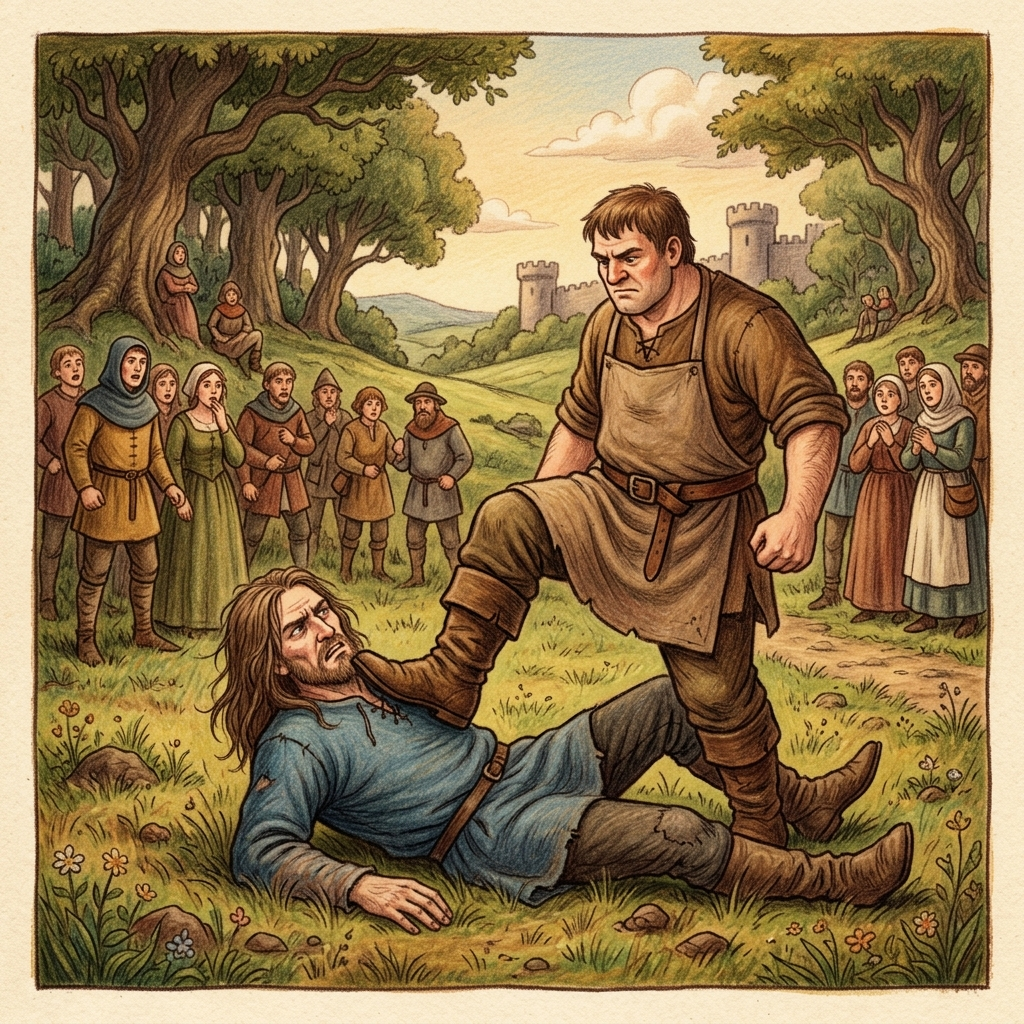
\includegraphics[width=0.6\linewidth]{vokab_300dpi/guergel_szene.png} \\
    \small\textit{De Géigner dréckt dem Veit de Fouss op d'Guergel / L'adversaire pose son pied sur la gorge de Veit / The opponent presses his foot on Veit's throat}
\end{center}


\textbf{16. Sou ass hien als Mäerder schëlleg gesprach ginn, a sollt deen aneren Dag duerch de Stréck stierwen.}\\
\textit{Sou} (Ainsi / Thus) \textit{ass hien... gesprach ginn} (a-t-il été déclaré / was he pronounced) \textit{als Mäerder} (comme meurtrier / as a murderer) \textit{schëlleg} (coupable / guilty), \textit{a sollt stierwen} (et devait mourir / and was to die) \textit{deen aneren Dag} (le lendemain / the next day) \textit{duerch de Stréck} (par la corde / by the rope/noose).\\
$\rightarrow$ Français : C'est ainsi qu'il a été déclaré coupable de meurtre, et devait mourir le lendemain par la corde.\\
$\rightarrow$ English : Thus, he was found guilty of murder, and was to die the next day by the noose.




\section[Beim Gaalgen]{Beim Gaalgen \\/ Au Gibet \\/ At the Gallows}

\noindent\textbf{Wéi jiddereen, deen zum Dout verurteelt gouf, duerft hien nach e leschte Wonsch äusseren. De Veit wollt op sengem leschte Wee zum Gaalgen seng Gei mathuelen. Wéi hien dunn schonns op der Leeder stoung, do op deem klengen Hiwwel, wou haut Parkierch steet, hunn d'Leit sech masseweis ronderëm gedrängt fir nozekucken wann hie géing um Gaalge baumelen; do huet hien ugefaangen op senger Gei ze spillen. Hien huet eng Melodie gespillt, déi d'Leit ronderëm gefesselt huet. Si si wéi ausser sech geroden duerch dës aussergewéinlech séiss-batter Kläng. Den Henker, deen uewen, prett op der Leeder stoung, huet d'Seel aus der Hand gelooss, an ass, ganz duercherneen erof geklomm.}\\[1.5em]

\begin{center}
    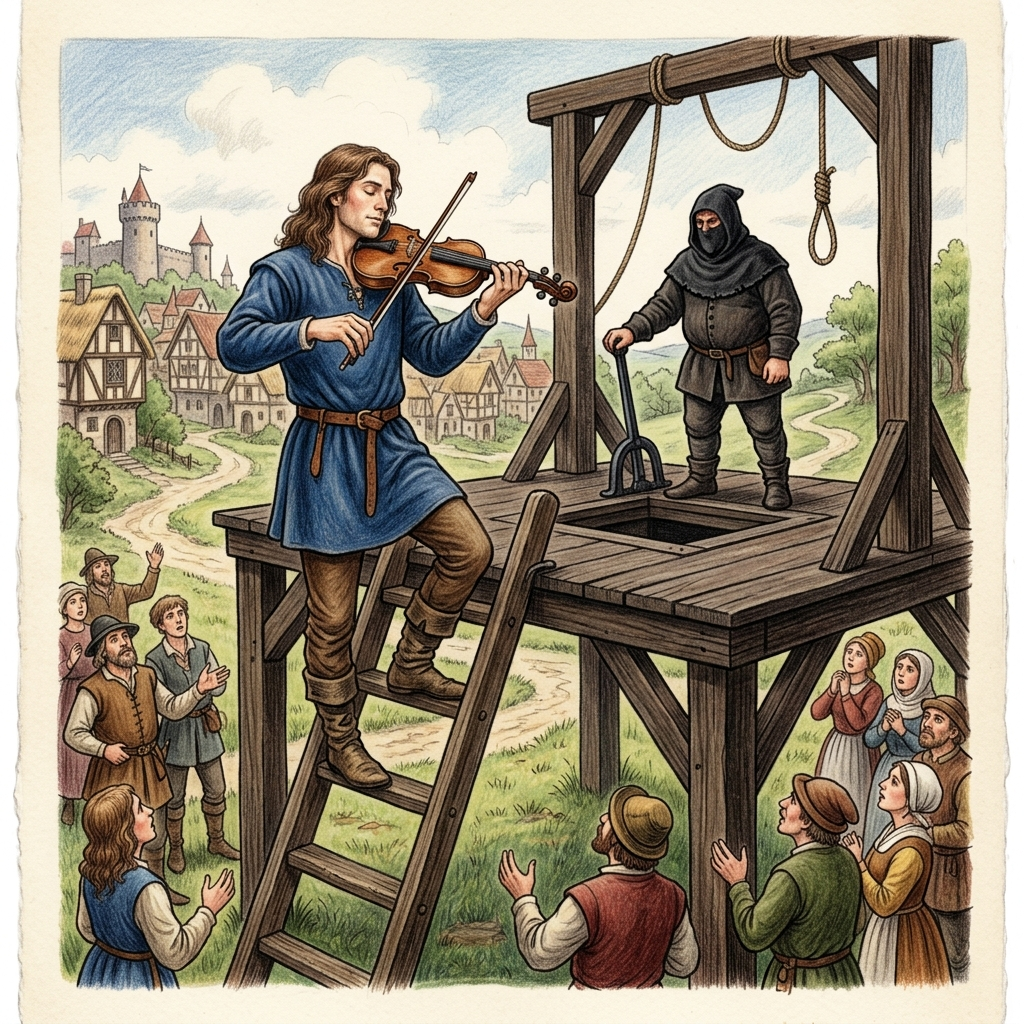
\includegraphics[width=0.6\linewidth]{vokab_300dpi/galgen_szene.png} \\
    \small\textit{De Veit spillt op senger Gei um Wee zum Gaalgen / Veit jouant du violon au gibet / Veit playing the violin on the gallows ladder}
\end{center}


\textbf{17. Wéi jiddereen, deen zum Dout verurteelt gouf, duerft hien nach e leschte Wonsch äusseren.}\\
\textit{Wéi jiddereen} (Comme tout le monde / Like everyone), \textit{deen zum Dout verurteelt gouf} (qui avait été condamné à mort / who was sentenced to death), \textit{duerft hien} (il pouvait / he was allowed to - past of \textit{däerfen}) \textit{nach e leschte Wonsch} (encore un dernier vœu / still a last wish) \textit{äusseren} (exprimer / to express).\\
$\rightarrow$ Français : Comme quiconque condamné à mort, il avait le droit d'exprimer un dernier vœu.\\
$\rightarrow$ English : Like everyone sentenced to death, he was allowed to express a last wish.\\[0.5em]

\textbf{18. De Veit wollt op sengem leschte Wee zum Gaalgen seng Gei mathuelen.}\\
\textit{De Veit} (Veit) \textit{wollt mathuelen} (voulait emporter / wanted to take along) \textit{seng Gei} (son violon / his violin) \textit{op sengem leschte Wee} (sur son dernier chemin / on his last path) \textit{zum Gaalgen} (vers le gibet / to the gallows).\\
$\rightarrow$ Français : Veit voulait emporter son violon sur son dernier chemin vers le gibet.\\
$\rightarrow$ English : Veit wanted to take his violin with him on his last path to the gallows.\\[0.5em]

\textbf{19. Wéi hien dunn schonns op der Leeder stoung, do op deem klengen Hiwwel, wou haut Parkierch steet, hunn d'Leit sech masseweis ronderëm gedrängt fir nozekucken wann hie géing um Gaalge baumelen; do huet hien ugefaangen op senger Gei ze spillen.}\\
\textit{Wéi hien dunn schonns} (Alors qu'il était déjà / When he was then already) \textit{op der Leeder stoung} (se tenait sur l'échelle / stood on the ladder), \textit{wou haut Parkierch steet} (où s'élève aujourd'hui l'église paroissiale / where the parish church stands today), \textit{hunn d'Leit sech masseweis gedrängt} (les gens se sont pressés en masse / people crowded in masses), \textit{fir nozekucken} (pour regarder / to watch) \textit{wann hie géing... baumelen} (quand il allait se balancer / when he would dangle), \textit{um Gaalge} (au gibet / on the gallows), \textit{do huet hien ugefaangen ze spillen} (c'est là qu'il a commencé à jouer / there he began to play).\\
$\rightarrow$ Français : Alors qu'il se tenait déjà sur l'échelle, là-bas sur la petite colline où s'élève aujourd'hui l'église paroissiale, les gens s'étaient pressés en masse pour regarder comment il allait se balancer au gibet ; c'est là qu'il commença à jouer de son violon.\\
$\rightarrow$ English : When he was already standing on the ladder, there on the small hill where the parish church stands today, the people crowded around in masses to watch him swing from the gallows; there he began to play on his violin.\\[0.5em]

\textbf{20. Hien huet eng Melodie gespillt, déi d'Leit ronderëm gefesselt huet.}\\
\textit{Hien huet... gespillt} (Il a joué / He played) \textit{eng Melodie} (une mélodie / a melody) \textit{déi} (qui / which) \textit{d'Leit ronderëm} (les gens autour / the people around) \textit{gefesselt huet} (a captivés / captivated).\\
$\rightarrow$ Français : Il a joué une mélodie qui a captivé les gens autour de lui.\\
$\rightarrow$ English : He played a melody that captivated the people around him.\\[0.5em]

\textbf{21. Si si wéi ausser sech geroden duerch dës aussergewéinlech séiss-batter Kläng.}\\
\textit{Si si} (Ils sont / They became) \textit{wéi ausser sech} (comme hors d'eux-mêmes / as if beside themselves) \textit{geroden} (devenus / got) \textit{duerch dës} (par ces / by these) \textit{aussergewéinlech séiss-batter Kläng} (sons exceptionnels doux-amers / extraordinary sweet-bitter sounds).\\
$\rightarrow$ Français : Ils sont devenus comme hors d'eux-mêmes à cause de ces sons exceptionnels, doux et amers.\\
$\rightarrow$ English : They became as if beside themselves because of these extraordinary, sweet-bitter sounds.\\[0.5em]

\textbf{22. Den Henker, deen uewen, prett op der Leeder stoung, huet d'Seel aus der Hand gelooss, an ass, ganz duercherneen erof geklomm.}\\
\textit{Den Henker} (Le bourreau / The executioner), \textit{deen} (qui / who) \textit{uewen, prett op der Leeder stoung} (se tenait en haut, prêt sur l'échelle / stood ready on the ladder), \textit{huet d'Seel aus der Hand gelooss} (a laissé tomber la corde de sa main / let the rope go from his hand), \textit{an ass... erof geklomm} (et est descendu / and climbed down), \textit{ganz duercherneen} (tout confus / very confused).\\
$\rightarrow$ Français : Le bourreau, qui se tenait en haut de l'échelle, prêt, a laissé tomber la corde de sa main et est descendu, tout confus.\\
$\rightarrow$ English : The executioner, who stood ready at the top of the ladder, let the rope go from his hand and climbed down, very confused.




\section[Den Danzrausch an d'Befreiung]{Den Danzrausch an d'Befreiung \\/ La folie de la danse \\/ The dancing frenzy}

\noindent\textbf{De Veit huet awer ëmmer nach weidergespillt, an et war, wéi wa Fonke vun senger Gei géife sprëtzen. Ëmmer méi schéin a sentimental gouf déi Musek an huet d'Leit ganz verzaubert. An, op eemol, huet hien ëmmer méi energesch gespillt, an d'Leit hunn ugefaangen ze danzen, am Ufank nach ganz lues awer dunn ëmmer méi séier bis si sech zu gudder Letzt wéi an Trance an engem wëllen Danz gedréit hunn. Männer, Fraen, Kanner an al Leit, si hunn all gedanzt. Dem Veit seng Famill an de Riichter hunn ënnert dem Gaalgen gedanzt an souguer d'Véi wat vun der Weed heem an de Stall gaangen ass, huet ugefaangen ze danzen. Alles wat zu Iechternach gelieft huet, war am Danzrausch. Sou ass de Veit gemittlech d'Leeder erof geklomm, an ass spillend duerch all déi danzend Leit gaangen, ëmmer méi wäit fort. Kee Mënsch war am Stand hien zeréckzehalen. Nach eng Zäit laang konnt een d'Téin vu senger Gei héieren, hie selwer war awer verschwonn a gouf ni méi an der Géigend gesinn. Déi Iechternacher awer hu weider gedanzt bis an d'Nuecht ran. An d'Famill vum Veit, sou heescht et an der So, konnt net méi ophalen mat danzen an huet nach e ganz Joer laang ëm d'Leeder vum Gaalgen gedanzt. Si ware schonns bis iwwer d'Knéien an de Buedem agesonk, wéi den hl. Willibrord zu Utrecht dovun héieren huet, an doropshin op Iechternach komm ass fir si vun dem Zauberdanz ze befreien.}\\[1.5em]

\begin{center}
    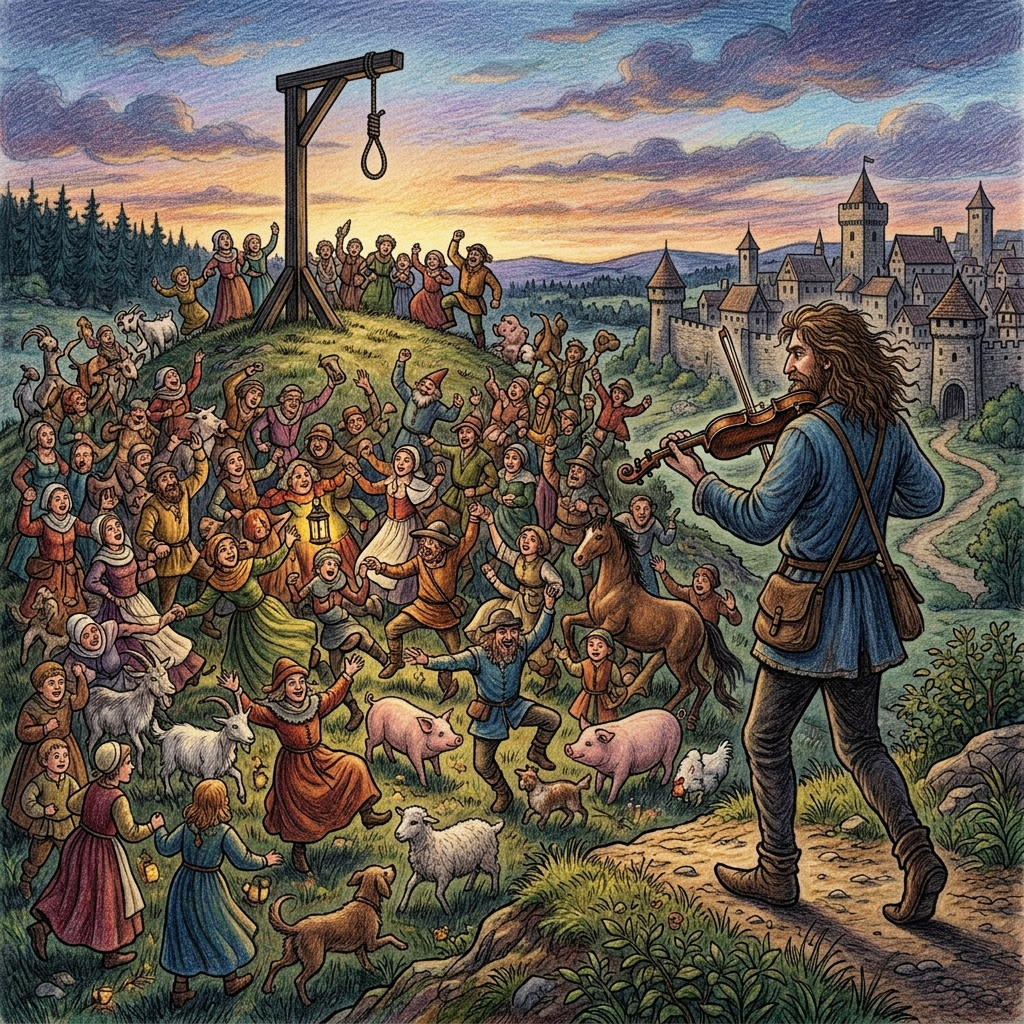
\includegraphics[width=0.6\linewidth]{vokab_300dpi/danz_szene.png} \\
    \small\textit{Den Danzrausch zu Iechternach / La folie de la danse à Echternach / The dancing frenzy in Echternach}
\end{center}


\textbf{23. De Veit huet awer ëmmer nach weidergespillt, an et war, wéi wa Fonke vun senger Gei géife sprëtzen.}\\
\textit{De Veit huet... weidergespillt} (Veit a continué à jouer / Veit continued playing) \textit{awer ëmmer nach} (cependant toujours / however still), \textit{an et war, wéi} (et c'était comme / and it was like) \textit{wa Fonke vun} (si des étincelles de / if sparks from) \textit{senger Gei} (son violon / his violin) \textit{géife sprëtzen} (allaient jaillir / would spray).\\
$\rightarrow$ Français : Mais Veit continuait de jouer, et c'était comme si des étincelles jaillissaient de son violon.\\
$\rightarrow$ English : But Veit kept on playing, and it was as if sparks were spraying from his violin.\\[0.5em]

\textbf{24. Ëmmer méi schéin a sentimental gouf déi Musek an huet d'Leit ganz verzaubert.}\\
\textit{Ëmmer méi schéin} (De plus en plus belle / More and more beautiful) \textit{gouf déi Musek} (devenait cette musique / became that music), \textit{an huet... verzaubert} (et a enchanté / and enchanted) \textit{d'Leit ganz} (les gens complètement / the people completely).\\
$\rightarrow$ Français : Cette musique devenait de plus en plus belle et mélancolique, et elle a complètement enchanté les gens.\\
$\rightarrow$ English : The music became more and more beautiful and sentimental, and it completely enchanted the people.\\[0.5em]

\textbf{25. An, op eemol, huet hien ëmmer méi energesch gespillt, an d'Leit hunn ugefaangen ze danzen, am Ufank nach ganz lues awer dunn ëmmer méi séier bis si sech zu gudder Letzt wéi an Trance an engem wëllen Danz gedréit hunn.}\\
\textit{An, op eemol} (Et, tout d'un coup / And, all of a sudden), \textit{huet hien... gespillt} (a-t-il joué / did he play) \textit{ëmmer méi energesch} (de plus en plus énergiquement / more and more energetically), \textit{an d'Leit hunn ugefaangen ze danzen} (et les gens ont commencé à danser / and the people began to dance), \textit{am Ufank nach ganz lues} (au début encore tout doucement / at the beginning still very slowly) \textit{awer dunn ëmmer méi séier} (mais ensuite de plus en plus vite / but then faster and faster) \textit{bis si sech... gedréit hunn} (jusqu'à ce qu'ils tournent / until they turned/twirled), \textit{zu gudder Letzt} (à la toute fin / in the end), \textit{wéi an Trance} (comme en transe / like in a trance) \textit{an engem wëllen Danz} (dans une danse sauvage / in a wild dance).\\
$\rightarrow$ Français : Et, tout à coup, il se mit à jouer de plus en plus énergiquement, et les gens commencèrent à danser, très lentement au début, puis de plus en plus vite, jusqu'à ce qu'ils tournent à la fin comme en transe dans une danse effrénée.\\
$\rightarrow$ English : And, all of a sudden, he played more and more energetically, and the people began to dance, very slowly at first, but then faster and faster until in the end they twirled like in a trance in a wild dance.\\[0.5em]

\textbf{26. Männer, Fraen, Kanner an al Leit, si hunn all gedanzt.}\\
\textit{Männer, Fraen, Kanner an al Leit} (Hommes, femmes, enfants et personnes âgées / Men, women, children and old people), \textit{si hunn all gedanzt} (ils ont tous dansé / they all danced).\\
$\rightarrow$ Français : Hommes, femmes, enfants et vieillards, ils dansaient tous.\\
$\rightarrow$ English : Men, women, children, and old people, they all danced.\\[0.5em]

\textbf{27. Dem Veit seng Famill an de Riichter hunn ënnert dem Gaalgen gedanzt an souguer d'Véi wat vun der Weed heem an de Stall gaangen ass, huet ugefaangen ze danzen.}\\
\textit{Dem Veit seng Famill} (La famille de Veit / Veit's family) \textit{an de Riichter} (et les juges / and the judges) \textit{hunn gedanzt} (ont dansé / danced) \textit{ënnert dem Gaalgen} (sous le gibet / under the gallows), \textit{an souguer d'Véi} (et même le bétail / and even the cattle) \textit{wat} (qui / which - relative pronoun) \textit{vun der Weed heem an de Stall gaangen ass} (est rentré du pâturage à l'étable / went home from the pasture into the stable), \textit{huet ugefaangen ze danzen} (a commencé à danser / began to dance).\\
$\rightarrow$ Français : La famille de Veit et les juges dansaient sous le gibet, et même le bétail qui rentrait du pâturage vers l'étable commença à danser.\\
$\rightarrow$ English : Veit's family and the judges danced under the gallows, and even the cattle that went home from the pasture into the stable began to dance.\\[0.5em]

\textbf{28. Alles wat zu Iechternach gelieft huet, war am Danzrausch.}\\
\textit{Alles} (Tout / Everything) \textit{wat zu Iechternach gelieft huet} (qui vivait à Echternach / that lived in Echternach), \textit{war am Danzrausch} (était en transe de danse / was in a dancing frenzy).\\
$\rightarrow$ Français : Tout ce qui vivait à Echternach était pris d'une frénésie de danse.\\
$\rightarrow$ English : Everything that lived in Echternach was in a dancing frenzy.\\[0.5em]

\textbf{29. Sou ass de Veit gemittlech d'Leeder erof geklomm, an ass spillend duerch all déi danzend Leit gaangen, ëmmer méi wäit fort.}\\
\textit{Sou ass de Veit... erof geklomm} (Ainsi Veit est descendu / Thus Veit climbed down) \textit{gemittlech} (tranquillement / calibre) \textit{d'Leeder} (de l'échelle / the ladder), \textit{an ass... gaangen} (et est allé / and went) \textit{spillend} (en jouant / playing) \textit{duerch all déi danzend Leit} (à travers tous ces gens dansants / through all those dancing people), \textit{ëmmer méi wäit fort} (de plus en plus loin / further and further away).\\
$\rightarrow$ Français : Ainsi, Veit descendit tranquillement de l'échelle et passa en jouant à travers la foule dansante, s'éloignant de plus en plus.\\
$\rightarrow$ English : Thus, Veit calmly climbed down the ladder and walked playing through all the dancing people, further and further away.\\[0.5em]

\textbf{30. Kee Mënsch war am Stand hien zeréckzehalen.}\\
\textit{Kee Mënsch} (Aucun homme, personne / No human, nobody) \textit{war am Stand} (était capable / was in a position, able) \textit{hien zeréckzehalen} (de le retenir / to hold him back - from \textit{zeréckhalen}).\\
$\rightarrow$ Français : Personne n'était en mesure de le retenir.\\
$\rightarrow$ English : Nobody was able to hold him back.\\[0.5em]

\textbf{31. Nach eng Zäit laang konnt een d'Téin vu senger Gei héieren, hie selwer war awer verschwonn a gouf ni méi an der Géigend gesinn.}\\
\textit{Nach eng Zäit laang} (Pendant encore un certain temps / For a while longer) \textit{konnt een} (pouvait-on / could one) \textit{d'Téin} (les sons / the sounds) \textit{vu senger Gei héieren} (entendre de son violon / hear of his violin), \textit{hie selwer war awer verschwonn} (mais lui-même avait disparu / he himself however had disappeared - equivalent to \textit{verschwonnen}), \textit{a gouf ni méi... gesinn} (et ne fut plus jamais vu / and was never seen again) \textit{an der Géigend} (dans la région / in the area).\\
$\rightarrow$ Français : Pendant un certain temps, on pouvait encore entendre les sons de son violon, mais lui-même avait disparu et ne fut plus jamais revu dans la région.\\
$\rightarrow$ English : For a while longer, one could still hear the sounds of his violin, but he himself had disappeared and was never seen in the area again.\\[0.5em]

\textbf{32. Déi Iechternacher awer hu weider gedanzt bis an d'Nuecht ran.}\\
\textit{Déi Iechternacher awer} (Mais les habitants d'Echternach / But the people of Echternach) \textit{hu weider gedanzt} (ont continué à danser / kept on dancing), \textit{bis an d'Nuecht ran} (tard dans la nuit / late into the night).\\
$\rightarrow$ Français : Les habitants d'Echternach, quant à eux, continuèrent à danser jusque tard dans la nuit.\\
$\rightarrow$ English : But the people of Echternach kept on dancing late into the night.\\[0.5em]

\textbf{33. An d'Famill vum Veit, sou heescht et an der So, konnt net méi ophalen mat danzen an huet nach e ganz Joer laang ëm d'Leeder vum Gaalgen gedanzt.}\\
\textit{An d'Famill vum Veit} (Et la famille de Veit / And Veit's family), \textit{sou heescht et} (ainsi dit-on / so it is said) \textit{an der So} (dans la légende / in the legend), \textit{konnt net méi ophalen} (ne pouvait plus s'arrêter / could not stop anymore) \textit{mat danzen} (de danser / dancing), \textit{an huet gedanzt} (et a dansé / and danced) \textit{nach e ganz Joer laang} (encore pendant une année entière / for a whole year longer) \textit{ëm d'Leeder} (autour de l'échelle / around the ladder) \textit{vum Gaalgen} (du gibet / of the gallows).\\
$\rightarrow$ Français : Et la famille de Veit, raconte la légende, ne pouvait plus s'arrêter de danser et dansa encore pendant une année entière autour de l'échelle du gibet.\\
$\rightarrow$ English : And Veit's family, so the legend goes, could no longer stop dancing and danced for a whole year around the ladder of the gallows.\\[0.5em]

\textbf{34. Si ware schonns bis iwwer d'Knéien an de Buedem agesonk, wéi den hl. Willibrord zu Utrecht dovun héieren huet, an doropshin op Iechternach komm ass fir si vun dem Zauberdanz ze befreien.}\\
\textit{Si ware schonns} (Ils étaient déjà / They were already), \textit{bis iwwer d'Knéien} (jusqu'au-dessus des genoux / to above their knees), \textit{an de Buedem agesonk} (enfoncés dans le sol / sunk into the ground - equivalent to \textit{agesonken}), \textit{wéi den hl. Willibrord} (quand saint Willibrord / when St. Willibrord) \textit{zu Utrecht dovun héieren huet} (en a entendu parler à Utrecht / heard of it in Utrecht), \textit{an doropshin} (et là-dessus / and thereupon) \textit{op Iechternach komm ass} (est venu à Echternach / came to Echternach), \textit{fir si... ze befreien} (pour les libérer / to free them) \textit{vun dem Zauberdanz} (de la danse magique / from the magic dance).\\
$\rightarrow$ Français : Ils s'étaient déjà enfoncés dans le sol jusqu'au-dessus des genoux lorsque saint Willibrord l'apprit à Utrecht et se rendit à Echternach pour les délivrer de cette danse magique.\\
$\rightarrow$ English : They had already sunk into the ground up to above their knees when Saint Willibrord heard of it in Utrecht and came to Echternach to free them from the magic dance.

\begin{center}
    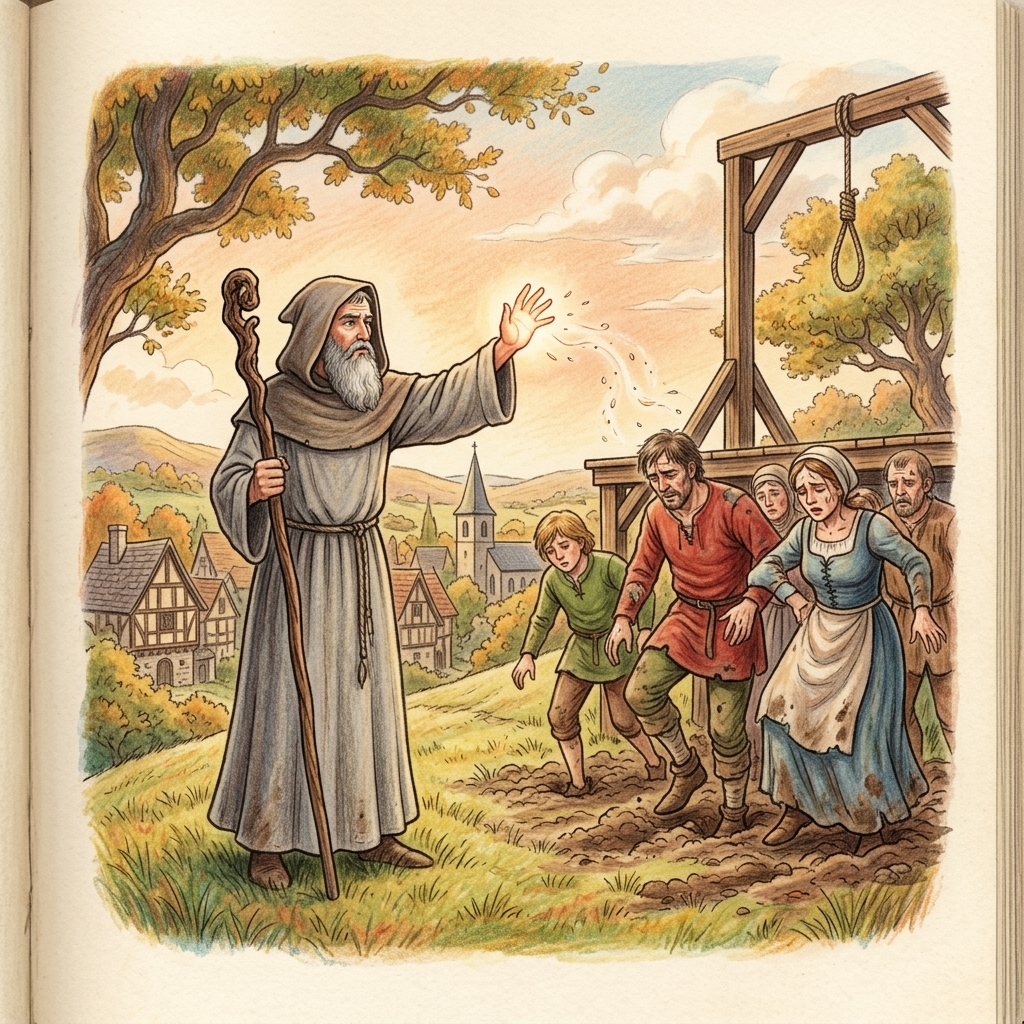
\includegraphics[width=0.6\linewidth]{vokab_300dpi/willibrord_befreiung.png} \\
    \small\textit{Den hellege Willibrord befreit d'Leit vum Zauberdanz / Saint Willibrord libère la foule de la danse magique / Saint Willibrord frees the crowd from the magic dance}
\end{center}


\section[De kompletten Text op Lëtzebuergesch]{De kompletten Text op Lëtzebuergesch \\/ Le texte complet en luxembourgeois \\/ The complete text in Luxembourgish}


\setlength{\parskip}{0pt}%
\setlength{\intextsep}{4pt}%
\setlength{\columnsep}{9pt}%

\begin{wrapfigure}{r}{0.25\textwidth}
  \centering
  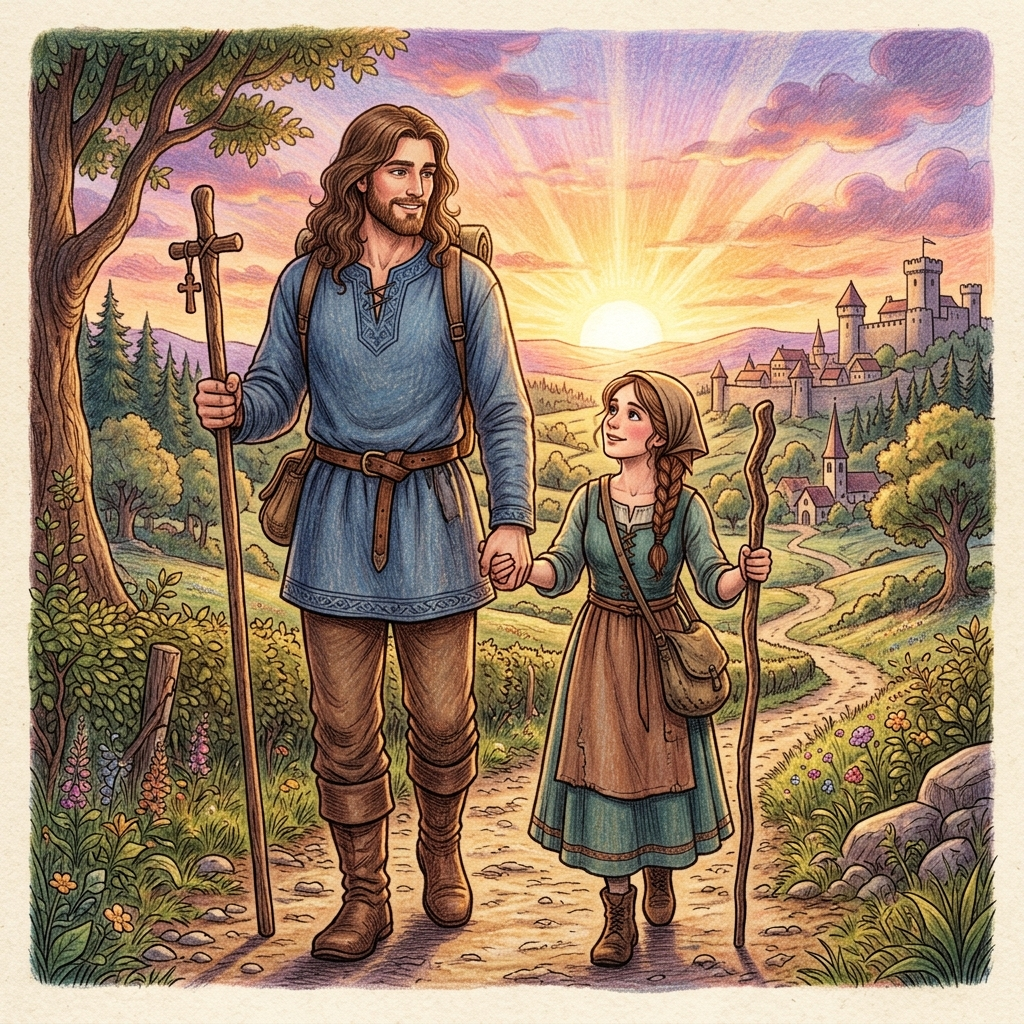
\includegraphics[width=\linewidth]{vokab_300dpi/pilger_wee.png}
\end{wrapfigure}
Zu der Zäit vum hellege Willibrord huet e jonke Mann zu Iechternach gewunnt.
Säin Numm war Veit, a well hien sou grouss war, gouf hien och "de Laange Veit" genannt.
Hie war, zesummen mat senger Fra, viru kuerzem, zum Chrëschtentum iwwergetrueden an si waren an d'Hellegt Land gepilgert.
Et waren elo schonns 10 Joer vergaangen, dass si fort waren, a well an Iechternach kee méi eppes vun hinnen héieren hat, hunn d'Leit geduecht, si wieren gestuerwen.
Doropshin huet hir Famill all hir Saachen ënnert sech opgedeelt.
Et war eng grouss Iwwerraschung, wéi, am Joer 729 op Ouschteren, de Laange Veit onverhofft rëm zu Iechternach opgetaucht ass.
Awer, a sengem Gesiicht, wat soss ëmmer sou gestraalt huet, stoung Trauer:
Seng gutt Fra war op der laanger Rees gestuerwen.
Si war souguer ëmbruecht ginn.
An hie selwer hat guer näischt méi, ausser engem komeschen, onbekannten Instrument: enger Gei.

\begin{wrapfigure}{l}{0.25\textwidth}
  \centering
  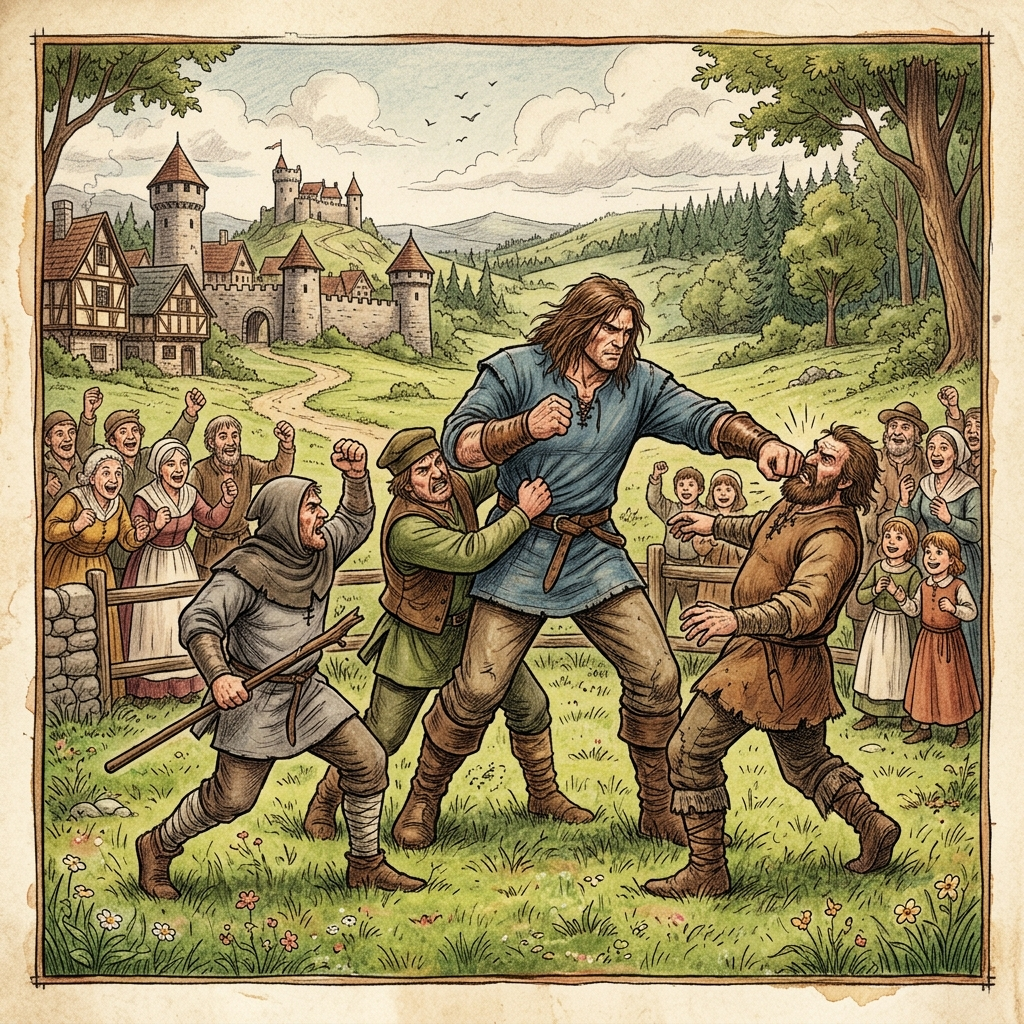
\includegraphics[width=\linewidth]{vokab_300dpi/duell_szene.png}
\end{wrapfigure}
Natierlech wollt de Veit säi Besëtz rëm zréck hunn, an dofir huet seng Famill beschloss hien als Mäerder unzekloen: Hien hätt seng Fra op der Rees ermuert.
Zu der Zäit war et de Gebrauch, dass esou eng Uklo duerch en Zweekampf ënnerstëtzt ginn ass.
Dësen Duell huet op Péngschtméindeg stattfonnt.
Dräi der stäerkste Männer haten sech bereet erkläert fir géint de Veit unzetrieden.
Schonns an der 1. Ronn, goung hien zu Buedem.
Wéi säi Géigner him dunn och nach de Fouss op d'Guergel gedréckt huet, huet hie missen opginn.
Sou ass hien als Mäerder schëlleg gesprach ginn, a sollt deen aneren Dag duerch de Stréck stierwen.
Wéi jiddereen, deen zum Dout verurteelt gouf, duerft hien nach e leschte Wonsch äusseren.
De Veit wollt op sengem leschte Wee zum Gaalgen seng Gei mathuelen.

\begin{wrapfigure}{r}{0.5\textwidth}
	\centering
	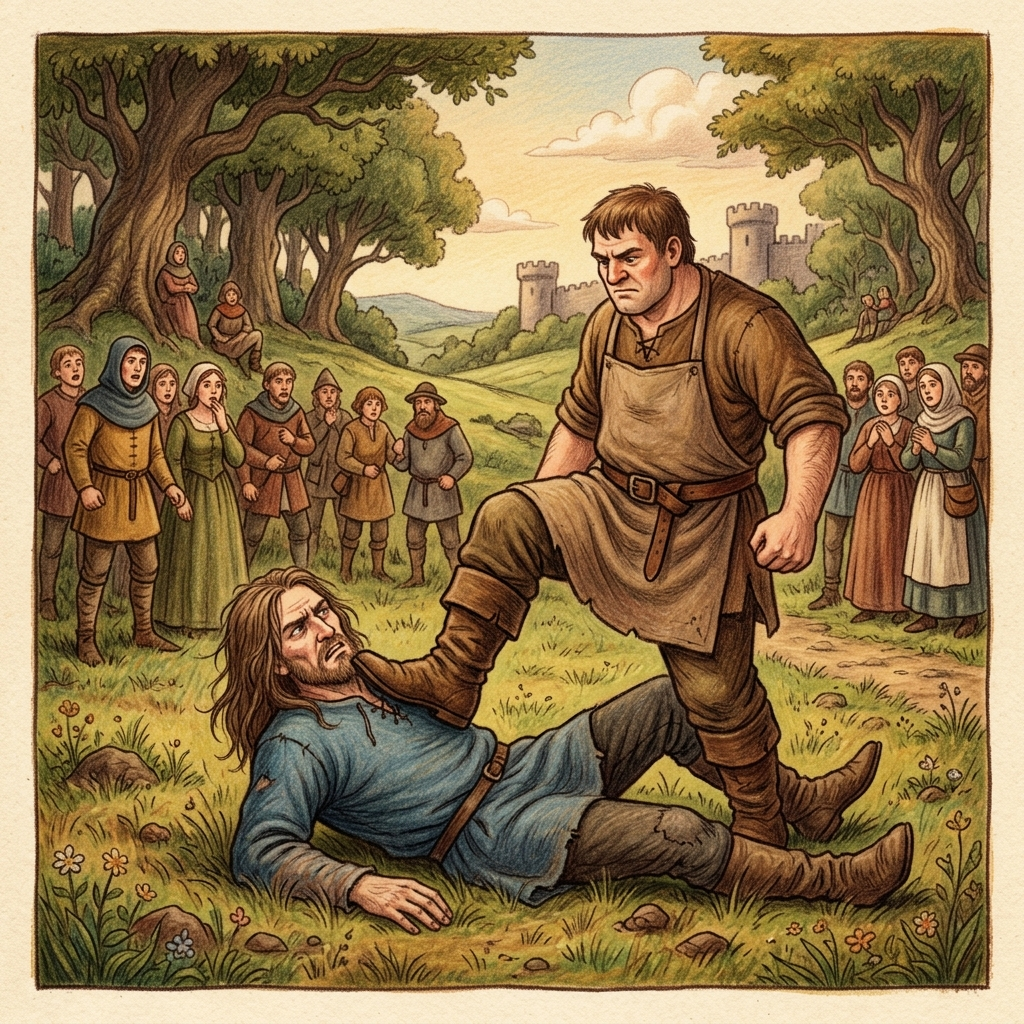
\includegraphics[width=0.48\linewidth]{vokab_300dpi/guergel_szene.png}
	  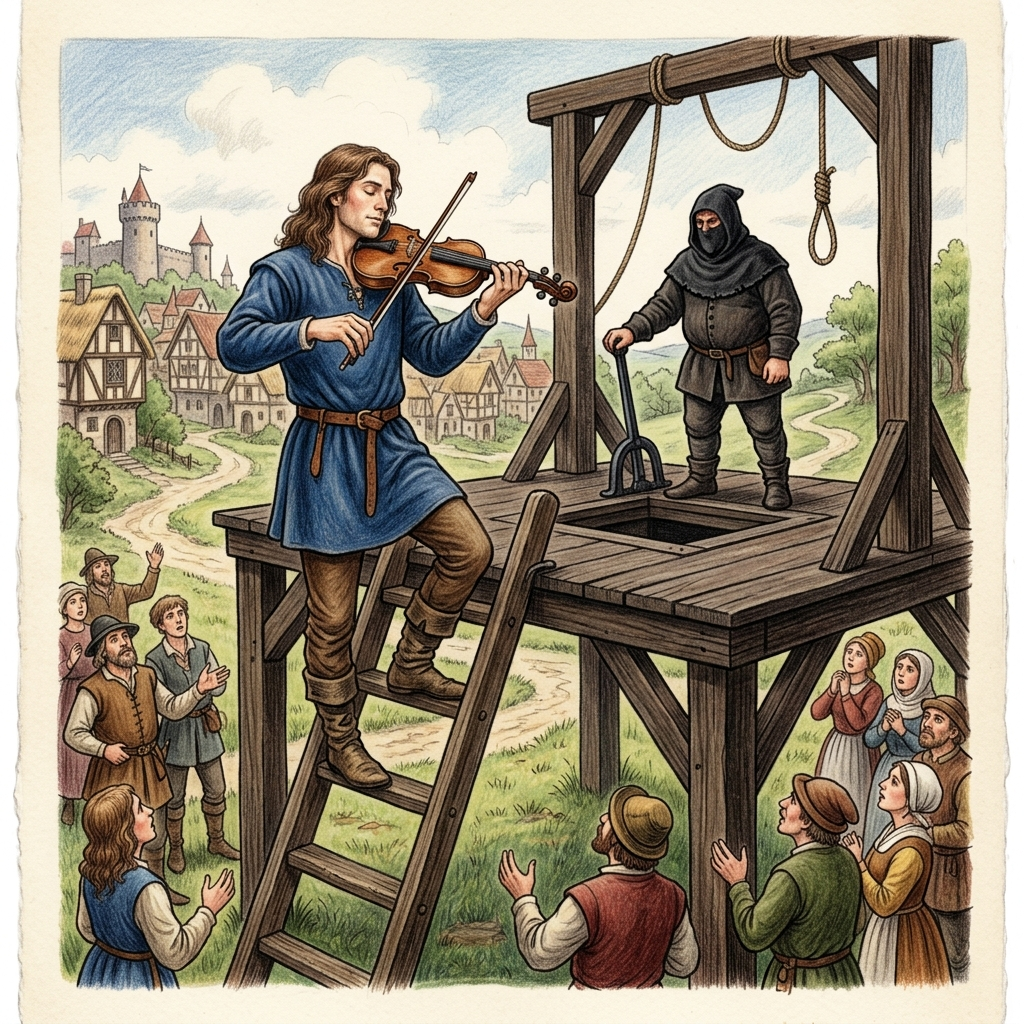
\includegraphics[width=0.48\linewidth]{vokab_300dpi/galgen_szene.png}
\end{wrapfigure}

Wéi hien dunn schonns op der Leeder stoung, do op deem klengen Hiwwel, wou haut Parkierch steet, hunn d'Leit sech masseweis ronderëm gedrängt fir nozekucken wann hie géing um Gaalge baumelen; do huet hien ugefaangen op senger Gei ze spillen.
Hien huet eng Melodie gespillt, déi d'Leit ronderëm gefesselt huet.
Si si wéi ausser sech geroden duerch dës aussergewéinlech séiss-batter Kläng.
Den Henker, deen uewen, prett op der Leeder stoung, huet d'Seel aus der Hand gelooss, an ass, ganz duercherneen erof geklomm.

\begin{wrapfigure}{l}{0.25\textwidth}
	\centering
	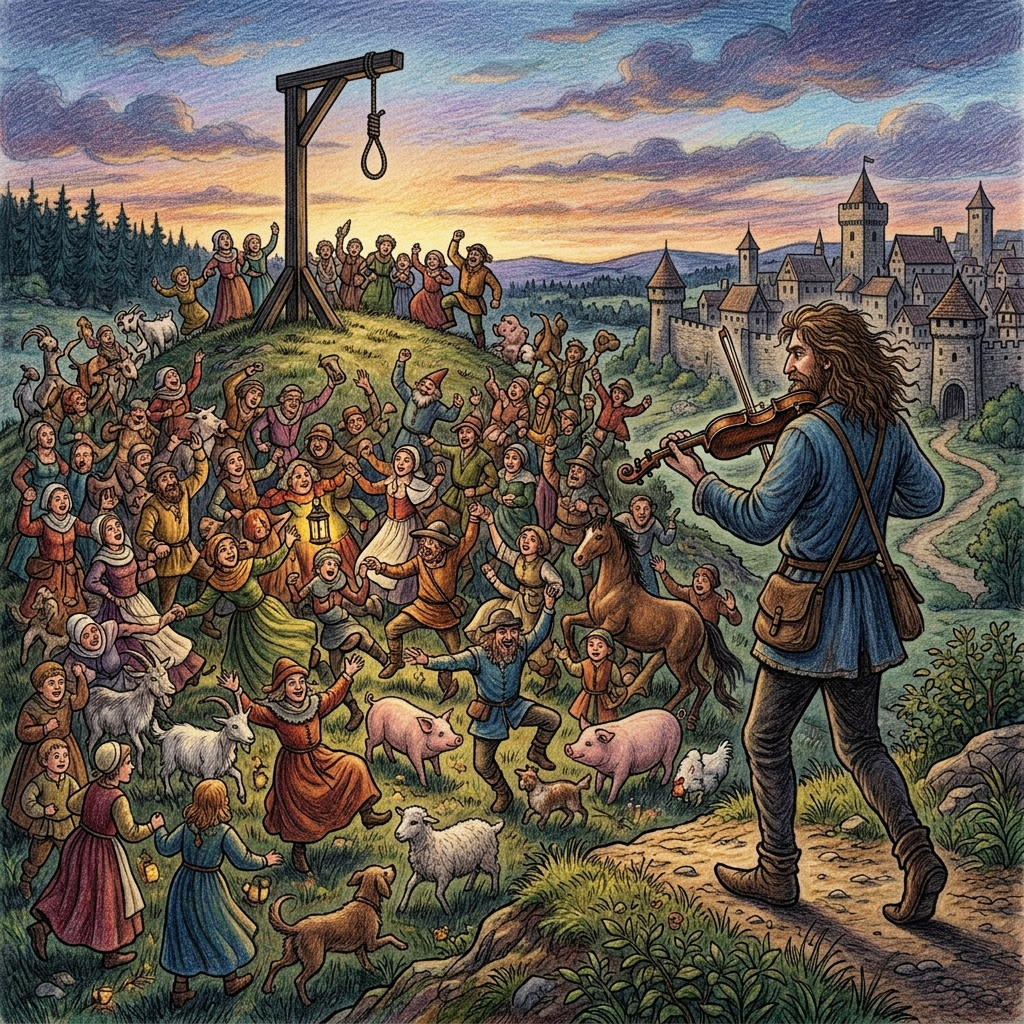
\includegraphics[width=\linewidth]{vokab_300dpi/danz_szene.png}
\end{wrapfigure}
De Veit huet awer ëmmer nach weidergespillt, an et war, wéi wa Fonke vun senger Gei géife sprëtzen.
Ëmmer méi schéin a sentimental gouf déi Musek an huet d'Leit ganz verzaubert.
An, op eemol, huet hien ëmmer méi energesch gespillt, an d'Leit hunn ugefaangen ze danzen, am Ufank nach ganz lues awer dunn ëmmer méi séier bis si sech zu gudder Letzt wéi an Trance an engem wëllen Danz gedréit hunn.
Männer, Fraen, Kanner an al Leit, si hunn all gedanzt.
Dem Veit seng Famill an de Riichter hunn ënnert dem Gaalgen gedanzt an souguer d'Véi wat vun der Weed heem an de Stall gaangen ass, huet ugefaangen ze danzen.

\begin{wrapfigure}{r}{0.25\textwidth}
	\centering
	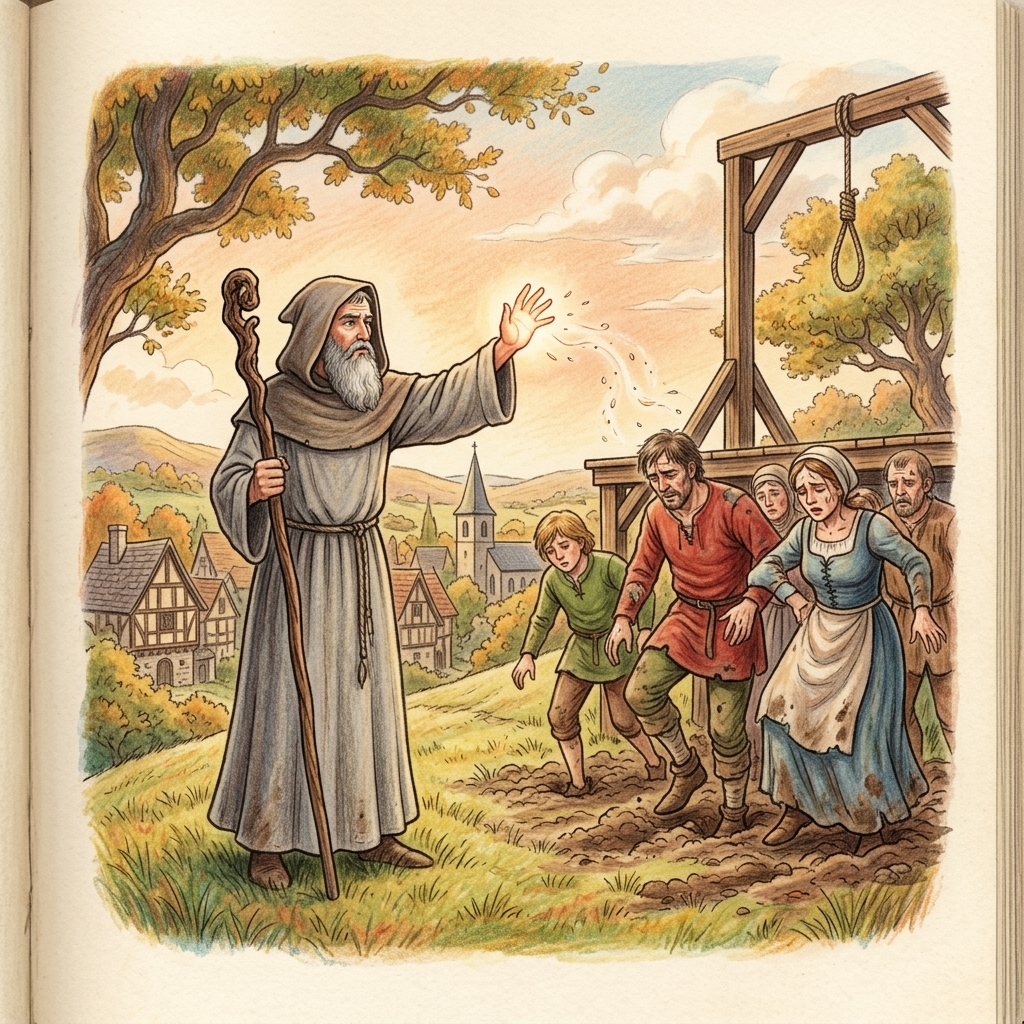
\includegraphics[width=\linewidth]{vokab_300dpi/willibrord_befreiung.png}
\end{wrapfigure}
Alles wat zu Iechternach gelieft huet, war am Danzrausch.

Sou ass de Veit gemittlech d'Leeder erof geklomm, an ass spillend duerch all déi danzend Leit gaangen, ëmmer méi wäit fort.
Kee Mënsch war am Stand hien zeréckzehalen.
Nach eng Zäit laang konnt een d'Téin vu senger Gei héieren, hie selwer war awer verschwonn a gouf ni méi an der Géigend gesinn.
Déi Iechternacher awer hu weider gedanzt bis an d'Nuecht ran.
An d'Famill vum Veit, sou heescht et an der So, konnt net méi ophalen mat danzen an huet nach e ganz Joer laang ëm d'Leeder vum Gaalgen gedanzt.
Si ware schonns bis iwwer d'Knéien an de Buedem agesonk, wéi den hl.\ Willibrord zu Utrecht dovun héieren huet, an doropshin op Iechternach komm ass fir si vun dem Zauberdanz ze befreien.


\vspace{0.3cm}

\section[Grammaire an Orthographie]{Grammaire an Orthographie \\/ Notes Grammaticales et Orthographe \\/ Grammar and Spelling Notes}

\subsection*{1. Orthographie / Orthographe / Spelling}
Verglach vum Text mat Standardalternativen : / Comparaison du texte avec les alternatives standardisées : / Comparison of the text with standard alternatives:

\begin{tabular}{ll}
    \toprule
    \textbf{Text Version} & \textbf{Alternative} \\
    \midrule
    sou & esou \\
    schonns & schonn \\
    dass & datt \\
    rëm & erëm \\
    verschwonn & verschwonnen \\
    \bottomrule
\end{tabular}

\subsection*{2. Prétérit vun de Modalverben / Le prétérit des verbes modaux / Preterite of modal verbs}
Notez la forme du prétérit du verbe modal \textbf{däerfen} dans la phrase 17 : / Note the past preterite form of the modal verb \textbf{däerfen} in sentence 17:
\begin{itemize}
    \item \textbf{duerft} (avait le droit de, pouvait / had the right to, was allowed to)
\end{itemize}

\subsection*{3. Passiv / Voix passive / Passive voice}
Le passif est formé avec le verbe auxiliaire \textbf{ginn} et le participe passé du verbe principal : / The passive is formed with the auxiliary verb \textbf{ginn} and the past participle of the main verb:
\begin{itemize}
    \item \textbf{gouf... genannt} (fut appelé / was called) - prétérit passif / preterite passive.
    \item \textbf{ënnerstëtzt ginn ass} (fut soutenu / was supported) - parfait passif / perfect passive.
    \item \textbf{ass... gesprach ginn} (fut déclaré, a été déclaré / was pronounced) - parfait passif / perfect passive.
    \item \textbf{war... ëmbruecht ginn} (avait été tué / had been killed) - plus-que-parfait passif / pluperfect passive.
\end{itemize}

\subsection*{4. Danzen (Danser / To dance)}
Le verbe \textbf{danzen} se conjugue comme suit au présent : / The verb \textbf{danzen} is conjugated as follows in the present tense:

\noindent
\begin{tabular}{ll c l l}
    \toprule
    \textbf{Pronom} & \textbf{Lëtzebuergesch} & \textbf{} & \textbf{Français} & \textbf{English} \\
    \midrule
    ech & danzen & $\rightarrow$ & Je danse & I dance \\
    du & danz & $\rightarrow$ & Tu danses & You dance \\
    hien / hatt / et & danzt & $\rightarrow$ & Il / Elle / On danse & He / She / It dances \\
    \midrule
    mir & danzen & $\rightarrow$ & Nous dansons & We dance \\
    dir & danzt & $\rightarrow$ & Vous dansez & You dance \\
    si & danzen & $\rightarrow$ & Ils / Elles dansent & They dance \\
    \bottomrule
\end{tabular}
\\[1em]
\textbf{Imperativ:} Danz! Danzt! (Danse ! Dansez ! / Dance!)

\subsection*{5. Spillen (Jouer / To play)}
Le verbe \textbf{spillen} se conjugue comme suit au présent : / The verb \textbf{spillen} is conjugated as follows in the present tense:

\noindent
\begin{tabular}{ll c l l}
    \toprule
    \textbf{Pronom} & \textbf{Lëtzebuergesch} & \textbf{} & \textbf{Français} & \textbf{English} \\
    \midrule
    ech & spillen & $\rightarrow$ & Je joue & I play \\
    du & spills & $\rightarrow$ & Tu joues & You play \\
    hien / hatt / et & spillt & $\rightarrow$ & Il / Elle / On joue & He / She / It plays \\
    \midrule
    mir & spillen & $\rightarrow$ & Nous jouons & We play \\
    dir & spillt & $\rightarrow$ & Vous jouez & You play \\
    si & spillen & $\rightarrow$ & Ils / Elles jouent & They play \\
    \bottomrule
\end{tabular}
\\[1em]
\textbf{Imperativ:} Spill! Spillt! (Joue ! Jouez ! / Play!)

\vspace{1.5cm}
\color{geminiBlue}\hrule height 1.5pt \vspace{0.5em}\color{black}
\section[Vokabulär: Nei Wierder]{Vokabulär: Nei Wierder \\/ Nouveau Vocabulaire \\/ New Vocabulary}

\begin{itemize}
    \item \textbf{d'Gei} (Pl.: d'Geien) $\rightarrow$ le violon (the violin)
    \item \textbf{de Gaalgen} (Pl.: de Gaalgen) $\rightarrow$ le gibet, la potence (the gallows)
    \item \textbf{de Stréck} (Pl.: d'Strécken) $\rightarrow$ la corde (the rope/noose)
    \item \textbf{de Géigner} (Pl.: d'Géigner) $\rightarrow$ l'adversaire (the opponent)
    \item \textbf{d'Guergel} (Pl.: d'Guergelen) $\rightarrow$ la gorge (the throat - colloquial)
    \item \textbf{schëlleg} $\rightarrow$ coupable (guilty)
\end{itemize}

\vspace{1em}

\begin{center}
    \begin{minipage}[t]{0.3\textwidth}
        \centering
        \textbf{Eng Gei}
        \vspace{0.5em}
        \framebox{\parbox{0.9\linewidth}{\centering
            \vspace{0.5cm}
            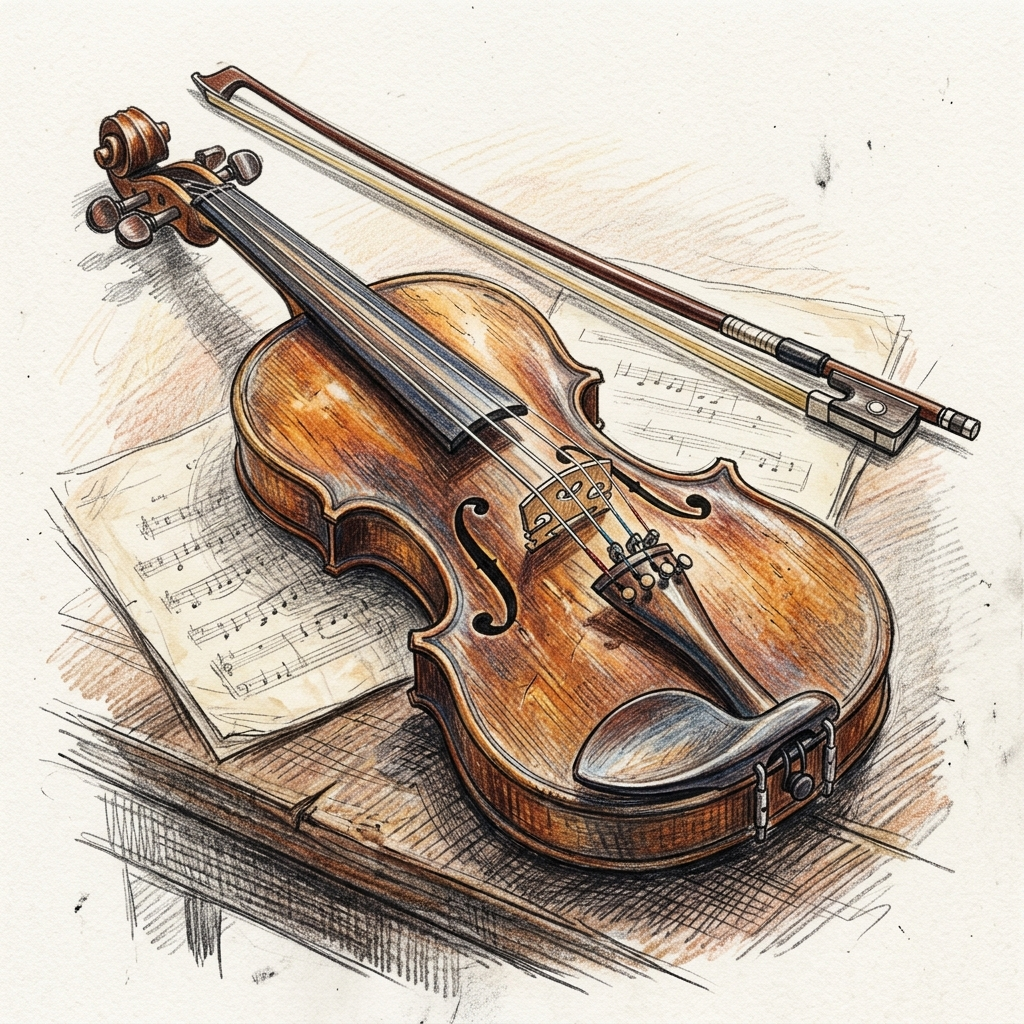
\includegraphics[width=0.9\linewidth]{vokab_300dpi/gei.png} \\
            \small\textit{D'Gei (Le violon / The violin)}
            \vspace{0.5cm}
        }}
    \end{minipage}
    \hfill
    \begin{minipage}[t]{0.3\textwidth}
        \centering
        \textbf{E Gaalgen}
        \vspace{0.5em}
        \framebox{\parbox{0.9\linewidth}{\centering
            \vspace{0.5cm}
            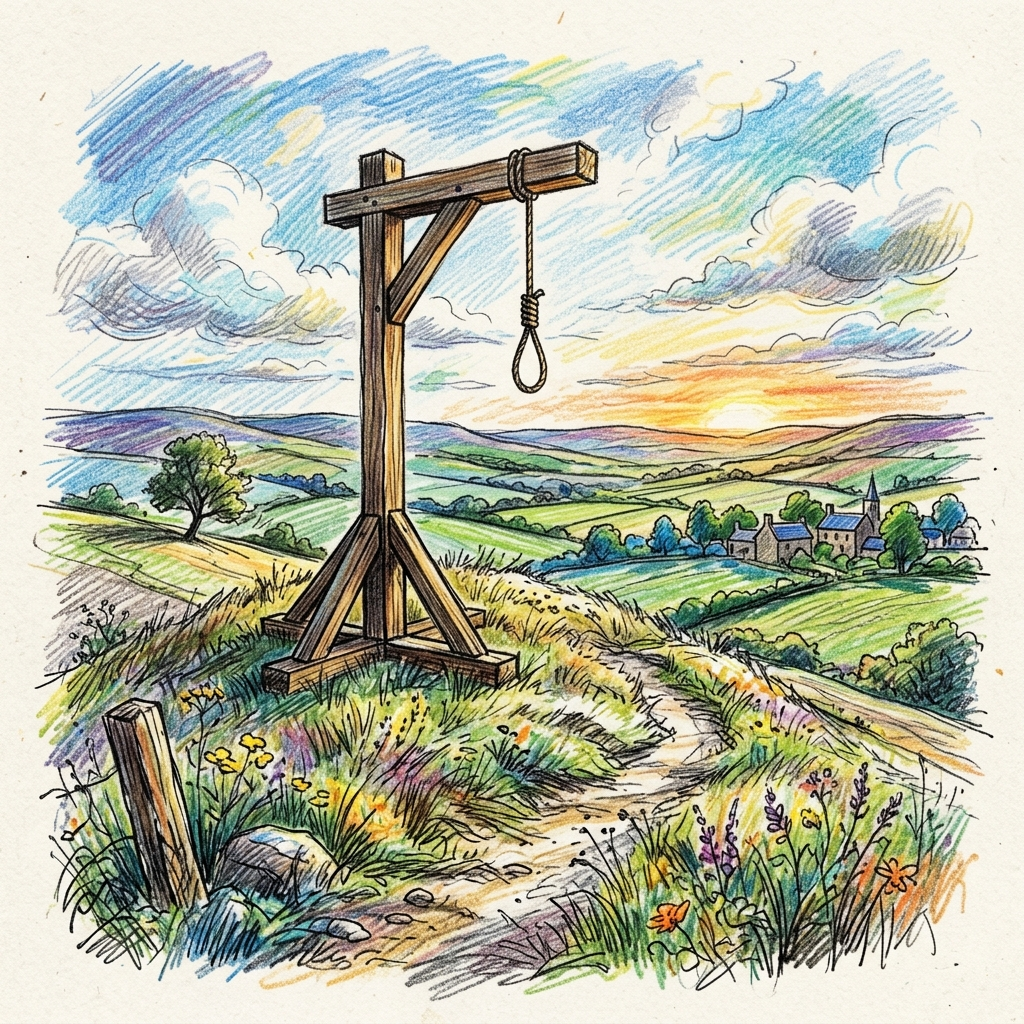
\includegraphics[width=0.9\linewidth]{vokab_300dpi/galgen.png} \\
            \small\textit{De Gaalgen (Le gibet / The gallows)}
            \vspace{0.5cm}
        }}
    \end{minipage}
    \hfill
    \begin{minipage}[t]{0.3\textwidth}
        \centering
        \textbf{Danzen}
        \vspace{0.5em}
        \framebox{\parbox{0.9\linewidth}{\centering
            \vspace{0.5cm}
            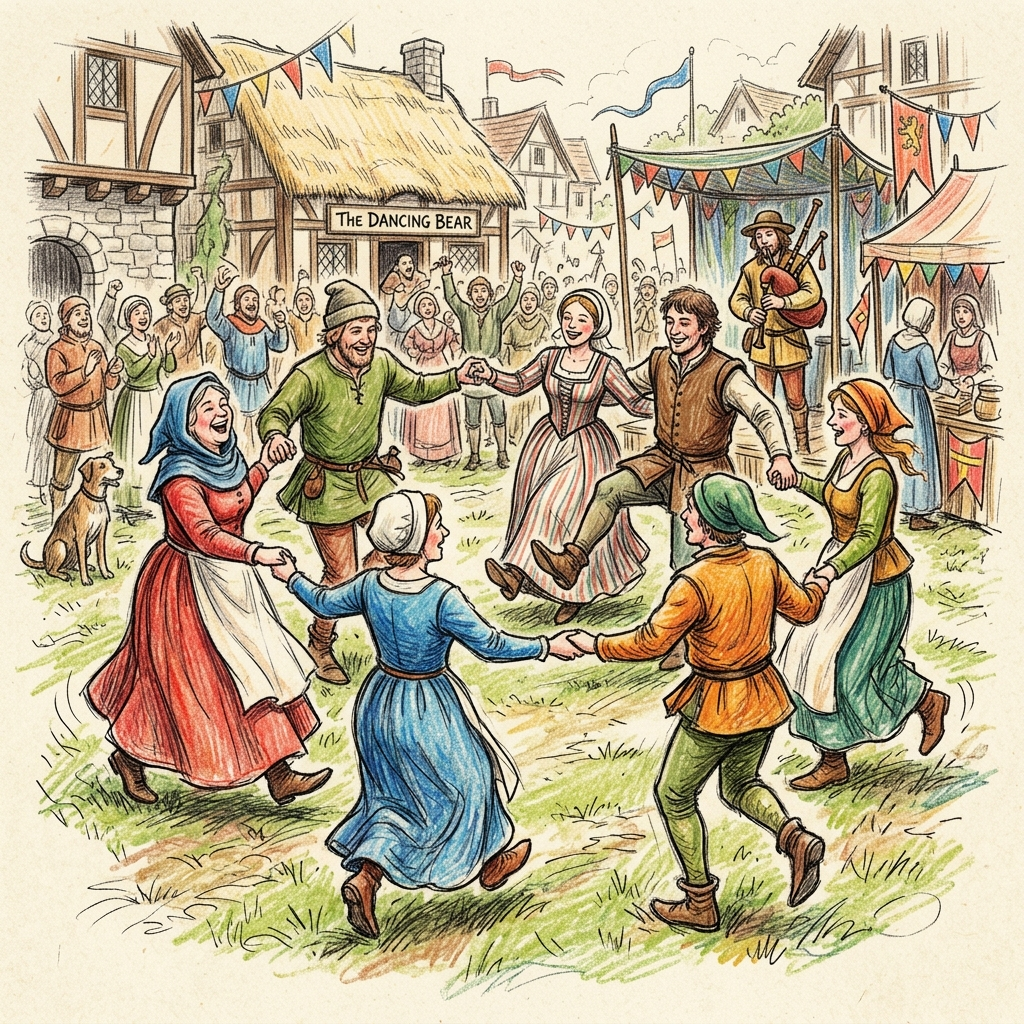
\includegraphics[width=0.9\linewidth]{vokab_300dpi/danzen.png} \\
            \small\textit{Danzen (Danser / To dance)}
            \vspace{0.5cm}
        }}
    \end{minipage}
\end{center}
